
% Identification of Actors and Their Roles
\section{Identification of Actors and Static Context Diagram}
% ==================================================

In order to define the system boundaries and understand the system's operation environment, it is necessary to define the different actors that interact with the AgriGov Market system. These actors represent the external world in our system: 


%------------------------------------------
\subsection{Farmer}

Farmers are agricultural producers who cultivate and supply agricultural products through the AgriGov platform.

\begin{itemize}
	\item Grow and provide fresh fruits and vegetables to the markets.
	\item Commercialization of agricultural production in an efficient manner.
	\item Management of agricultural farms by keeping product availability updated.
	\item Confirm or reject orders.
	\item Control of sales and revenue to make business decisions.
\end{itemize}

%------------------------------------------
\subsection{Buyer}

Buyers are individuals or organizations (retailers, wholesalers, restaurants, or end consumers) who purchase agricultural products via the platform.

\begin{itemize}
	\item Buyers include individual buyers, retailers and wholesalers looking for fresh products.
	\item Transparent purchase of products.
	\item Browse and search products on the platform.
	\item Tracking the delivery of products.
	\item Establishing long-term relationships with farmers.
	\item Moving from intermediaries to direct connection with farmers.
\end{itemize}

%------------------------------------------
\subsection{Transporter}

Transporters are logistics operators responsible for delivering agricultural products from farmers to buyers.

\begin{itemize}
	\item Carry products from farms to buyers.
	\item Viewing available delivery opportunities.
	\item Selection of delivery missions along their routes.
	\item Collection of products from farms.
	\item Providing status updates during transportation.
	\item Real-time tracking of farms.
\end{itemize}

%------------------------------------------
\subsection{Ministry}

The Ministry of Agriculture is the official governmental authority and owner of the AgriGov platform.

\begin{itemize}
	\item Oversees the food system.
	\item Establishment of rules ensuring fairness and transparency.
	\item Control of participation in the food system through approval and validation of farmers, buyers, and transporters.
	\item Definition of product categories used in the platform.
	\item Establishment of price references to prevent exploitation.
	\item Monitoring of production, distribution, and pricing of agricultural products.
	\item Support for shaping national agricultural policy.
	\item Protection of farmers and consumers through platform supervision.
\end{itemize}

%------------------------------------------
\subsection{Quality Inspector}

The Quality Inspector operates under the supervision of the Ministry of Agriculture and verifies product compliance.

\begin{itemize}
	\item Inspection of farms and collection points.
	\item Verification of product quality.
	\item Checking freshness, size, safety, and labeling of products.
	\item Comparison with government standards.
	\item Approval of products for listing when standards are met.
	\item Rejection of products that do not meet required standards.
	\item Protection of consumers from fraud.
	\item Assurance of fair competition among farmers.
\end{itemize}

%------------------------------------------
\subsection{Delivery Manager}

The Delivery Manager supervises and coordinates delivery operations.

\begin{itemize}
	\item Management of logistics operations.
	\item Assignment of delivery missions to transporters.
	\item Intervention in case of delivery problems or delays.
	\item Ensuring efficient product delivery.
	\item Minimization of delivery time and cost.
\end{itemize}

%------------------------------------------
\subsection{Payment System}

The Payment System is an external financial service integrated into the platform.

\begin{itemize}
	\item Facilitation of secure money transfer from buyer to farmer.
	\item Processing payments when orders are made.
	\item Verification of funds availability.
	\item Notification of users about transaction status.
	\item Protection of financial information through encryption.
	\item Support for digital trade operations.
\end{itemize}

%------------------------------------------
\subsection{Weather System}

The Weather System is an external service providing meteorological data.

\begin{itemize}
	\item Provide real-time weather forecasts.
	\item Support farmers in harvest and planting decisions.
	\item Assist transporters in avoiding weather-related delays.
	\item Alert users to extreme conditions (storms, frost, heatwaves).
	\item Enable better coordination of delivery schedules based on climate conditions.
\end{itemize}
%----------
\subsection{System Context Diagram}
\addcontentsline{toc}{section}{System Context Diagram}


According to Dennis et al. \cite{dennis2015}, a context diagram is a high-level graphical representation of a system that illustrates the system as a single process and defines its interactions with external entities. It establishes the system boundary and shows the flow of information between the system and its environment without revealing internal system processes. This type of diagram helps stakeholders understand the overall scope, external interfaces, and operational environment of the system.

\begin{figure}[H]
	\centering
	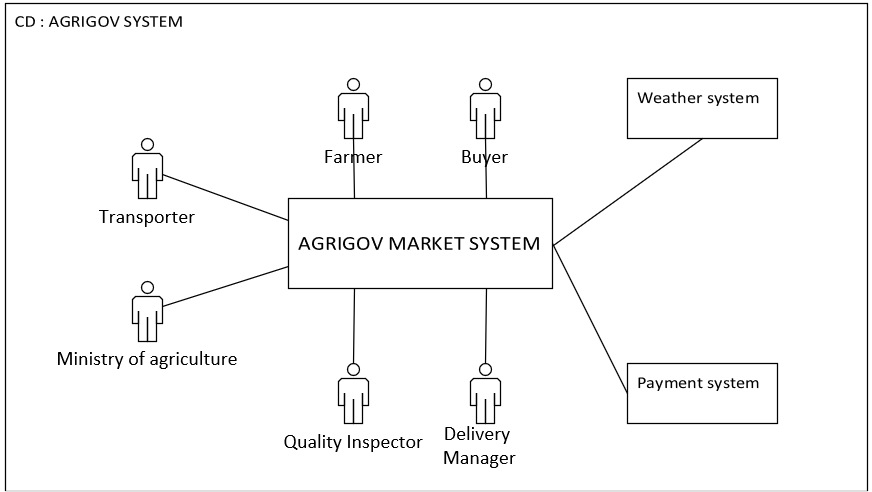
\includegraphics[width=1\textwidth]{images/diagrammes/DCS}
	\caption{AgriGov Market System Context Diagram}
	\label{fig:dcs}
\end{figure}

This diagram provides a global view of the system and helps identify all external actors and their interactions with the AgriGov Market platform. It serves as a foundation for further system analysis and design phases.